\section{CCS parsing and LTS generation}
\label{sec:parsing}

Given a set of action names, the set of CCS processes is defined by the following BNF grammar:

\begin{equation}\label{eq:ccs_bnf}
P ::= \emptyset \hspace{1 mm} | \hspace{1 mm} a.P_{1} \hspace{1 mm} | \hspace{1 mm} A \hspace{1 mm} | \hspace{1 mm}P_{1}+P_{2} \hspace{1 mm} |
\hspace{1 mm} P_{1} | P_{2} \hspace{1 mm} | \hspace{1 mm} P_{1}[b/a] \hspace{1 mm} | \hspace{1 mm} P_{1} \backslash a
\end{equation}

Two choices were considered for the problem of building a parser. The first choice was to build
a new parser, which required much more resources and the second choice was to define a grammar
and to use a parser generator (compiler-compiler, compiler generator) software to generate the parser source code.
In formal language theory, a context-free grammar (CFG) is a grammar in which every production 
rule has the form:
\[V \rightarrow w \]
where V e is a nonterminal symbol, and w is a string of terminal and/or nonterminal symbols 
(w can be empty). Obviously, the defined BNF grammar for describing the CCS process is a CFG. 
Deterministic context-free grammars (DCFGs) are grammars that can be recognized by a 
deterministic pushdown automaton or equivalently, grammars that can be recognized by a LR (left to right) parser. 
DCFGs are a proper subset of the context-free grammar family. Although, the defined grammar is 
a non-deterministic context-free grammar, modern parsers have a look ahead feature, which means that
the parser will not make a parsing decision until it reads ahead several tokens. This feature
alows us to use a parser generator software, that will generate LR or LL parser which is able to
recognize the non-deterministic grammar.

\subsection{Generating the parser}
ANTLR (ANother Tool for Language Recognition) \cite{ANTLRRef} is a parser generator that was used 
to generate the parser for the CCS grammar. ANTLR uses LL(*) parsing and also allows generating 
parsers, lexers, tree parsers and combined lexer parsers. It also automatically generates 
abstract syntax trees (AST), by providing operators and rewrite rules to guide the tree construction,
which can be further processed with a tree parser, to build an abstract model of the AST using some programming language.
A language is specified by using a context-free
grammar which is expressed using Extended Backus Naur Form (EBNF). In short, an LL parser is a 
top-down parser which parses the input from left to right and constructs a Leftmost derivation 
of the sentence. An LL parser is called an LL(*) parser if it is not restricted to a finite k 
tokens of lookahead, but can make parsing decisions by recognizing whether the following tokens
belong to a regular language. This is achieved by building temporary deterministic finite
automaton, which are maintained and used until the parser makes a decision. This feature and
some more optimization for the LL parser were published in recent years which made this kind 
of parser generators popular and favorable.

ANTLR was used to generate lexer, parser and a well defined AST which represents a tree representation 
of the abstract syntactic structure of the parsed sentence. The term abstract is used in a sense 
that the tree does not represent every single detail that exists in the language syntax, 
for example, parentheses are implicit in the tree structure. 
From a development point of view it is much easier to work with trees than with a list of recognized
tokens. One example of an AST is shown in  Fig. \ref{fig:ast_example} which is the result of parsing the expression: 

\begin{equation}\label{eq:ccs_example}
 A=( b.B \hspace{1 mm} | \hspace{1 mm} c.D \hspace{1 mm} + \hspace{1 mm} d.D )
\backslash \left\lbrace b, \hspace{1 mm} c \right\rbrace 
\end{equation}

\begin{figure}[!t]
\centering
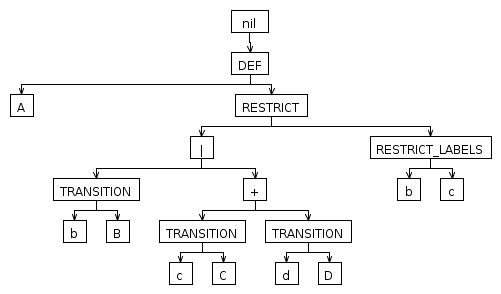
\includegraphics[width=3.5in]{ast_example}
\caption{AST Example}
\label{fig:ast_example}
\end{figure}

\subsection{CCS domain model and LTS graph generation}
Although working directly with ASTs and performing all algorithms on them is possible, it causes 
a limitation in future changes, where even a small change in the grammar and/or in the structure of the
generated ASTs causes a change in the implemented algorithms. Because of this,
a specific domain model is built along with a domain builder algorithm, which has corresponding
abstractions for all CCS operators, processes and actions. The input of the domain builder algorithm 
is an AST, and the output is a fully built domain model. The algorithms for constructing an LTS graph 
are implemented on the domain model because it is not expected for the domain model structure to 
change much in the future. The domain model is also a tree-like structure, so it is as easy to work with, 
as with the AST. 

The LTS generation algorithm is a recursive algorithm which traverses the tree structure of objects 
in the domain model and performs SOS rule every time it reaches an operation.
In this fashion all SOS transformation are performed on the domain and as result a new graph
structure is created which represents the LTS which can be easily exported to a file
in Aldebaran format.

\subsection{Workflow of operations}
In  Fig. \ref{fig:workflow} the workflow of all operations that are executed for constructing an LTS graph from a 
CCS expression are shown. Every operation is done as a standalone algorithm independent from the other operations,
that has input and output shown in the Figure. The modular design is deliberately chosen in order to help achieve better 
testing and maintenance of the source code. 

\begin{figure}[h]
\centering
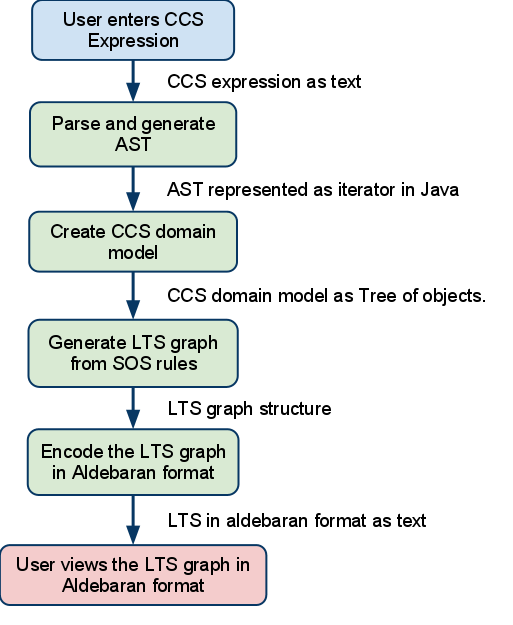
\includegraphics[height=3.0in]{workflow}
\caption{Workflow of all operations for producing an LTS graph from a CCS expression}
\label{fig:workflow}
\end{figure}
